\documentclass{article}
\usepackage{fullpage}
\usepackage{amsmath}
\usepackage{graphicx}
\usepackage{natbib}


% \DeclareMathOperator{\Sample}{Sample}
\let\vaccent=\v % rename builtin command \v{} to \vaccent{}
\renewcommand{\v}[1]{\ensuremath{\mathbf{#1}}} % for vectors
%\renewcommand{\v}[1]{\ensuremath{\mbox{\boldmath$ #1 $}}}
\newcommand{\gv}[1]{\ensuremath{\mbox{\boldmath$ #1 $}}}
% for vectors of Greek letters
\newcommand{\uv}[1]{\hat{\ensuremath{\mathbf{ #1 }}}} % for unit vector
\newcommand{\abs}[1]{\left| #1 \right|} % for absolute value
\newcommand{\avg}[1]{\left< #1 \right>} % for average
\let\underdot=\d % rename builtin command \d{} to \underdot{}
\renewcommand{\d}[2]{\frac{d #1}{d #2}} % for derivatives
\newcommand{\dd}[2]{\frac{d^2 #1}{d #2^2}} % for double derivatives
\newcommand{\pd}[2]{\frac{\partial #1}{\partial #2}}
% for partial derivatives
\newcommand{\pp}[2]{\frac{\partial^2 #1}{\partial #2^2}}
% for double partial derivatives
\newcommand{\grad}[1]{\v{\nabla} #1} % for gradient
\let\divsymb=\div % rename builtin command \div to \divsymb
\renewcommand{\div}[1]{\v{\nabla} \cdot #1} % for divergence
\newcommand{\curl}[1]{\v{\nabla} \times #1} % for curl



\title{A fully Lagrangian Dynamical Core for the Met Office NERC Cloud Model}
\author{G. Gibb, S. Boeing, D. Dritschel}


\begin{document}
\maketitle
\abstract{We describe the technical work carried out in the eCSE project `A fully Lagrangian Dynamical Core for the Met Office NERC Cloud Model', whose aim is to incorporate the `Moist Parcel in Cell` (MPIC) code into the Met Office Nerc Cloud Model (MONC). First we describe the modifications to MONC in order for it to be parcel-aware, then we outline the implementation of MPIC's physics into MONC. We then provide an in-depth comparison of MPIC with the newly developed code, and investigate how it scales to many thousands of MPI processes. Finally we discuss the limitations of the code, and future work to be carried out to mitigate these limitations. We found that the code can scale up to many thousands of cores for large problem sizes, although the main limiter of performance at scale are the Fourier Transform routines. Despite good MPI performance from the code, OpenMP performance is poor, achieving a speedup of only 3 on 12 threads. Overall, on a single node the new code performs better than MPIC does, carrying out more parcel operations per core per second.}
%\tableofcontents



\section{Introduction}

This report documents the technical work carried out in the eCSE project entitled `A fully Lagrangian dynamical core for the Met Office NERC Cloud Model'. The aim of this project was to implement the functionality of the `Moist parcel in cell' code developed by \citet{Dritschel2018} into the `Met Office NERC Cloud Model' \citep{Brown2015}. In this section we will describe the two aforementioned codes and the original proposed work. In the following section (Section \ref{development}) we will describe the development work carried out. We then describe scaling tests and comparisons with the original code in Section \ref{performance}. Finally, we summarise the outputs from the project and discuss future work in Section \ref{discussion}.

\subsection{Moist Parcel in Cell}

The `Moist Parcel in Cell' code (hereby MPIC) is a Lagrangian fluid dynamics code which models moist convection and cloud development. It achieves this by representing the fluid as a large number of `moist parcels' containing various properties such as buoyancy, vorticity and humidity. Whilst the code is Lagrangian, a gridded approach is used in order to solve for the parcel velocity and vorticity tendency. This is achieved by trilinearly interpolating the parcel properties onto grids, solving for the velocity and vorticity tendency on these grids, then trlinearly interpolating these gridded values back onto the parcels. The parcel-based approach has many benefits over a purely grid-based approach, such as allowing for explicit sub-grid representation, a velocity field that is undamped by numerical diffusion down to the grid scale and it is exactly conservative. The approach also allows for a natural description of mixing, whereby parcels can split into two and merge together.

MPIC is written in Fortran and is parallelised using OpenMP. This imposes a limitation on both the scalability of the code (due to it being limited to only a small number of cores), and more crucially on the number of parcels (and thus indirectly the grid resolution) that can be used due to the memory limitations of a single node. MPIC at present uses dimensionless (normalised) units. MPIC evolves the parcels via a fourth-order Runge Kutta integrator (RK4). Figure \ref{flowchart} shows a flowchart for the basic struture of MPIC.


\subsection{Met Office NERC Cloud Model}

The `Met Office NERC Cloud Model' (hereby MONC) is an Eulerian fluid dynamics code that simulates cloud microphysics. MONC was designed to supersede the older Met Office Large Eddy Model (LEM), which did not scale beyond 512 cores. As such it can be regarded as a complete re-write of the LEM. It was designed to be easy to modify and implement new functionality into. It employs a ``plug-in'' architecture whereby it consists of a number of independent `components' which can be selected and run in a specific order at runtime. Components can be switched on/off to add/remove functionality, or swapped out with other components to provide - for example - different solvers. This allows for a highly customisable code that is easy to develop new functionalty for.

MONC is organised into three different parts, the \emph{Model Core}, the \emph{Model State} and the \emph{Components}. The Model Core consists of the core functionality of MONC, including how it handles components, reading in configuration files, and functions/subroutines common to all components (e.g. haloswapping). The Model State contains the data describing the state of the simulation, such as the grids, as well as various other variables such as the time, timestep and other runtime-specific quantities. The components, which are called once per timestep in a user-defined order, perform actions on the data contained within the Model State. MONC is parallelised using MPI, and scales up to 32,768 cores. It is spatially decomposed in the $x$ and $y$ directions. Unlike MPIC, it uses an Eulerian integrator to evolve its Model State.

MONC also has an \emph{I/O server} which permits real-time in-situ analysis of the simulation data. This works by having a number of processes set aside (typically one per node) for analytics and I/O. The compute processes periodically asynchronously send data to the I/O Servers, which then perform any necessary reduction operations on the data and write the results to disk. This setup allows the compute processes to concentrate on carrying out the simulation work, whilst the I/O servers can take on the burden of analysis and I/O. Figure \ref{flowchart} shows a flowchart for the basic struture of MONC.

\begin{figure}
  \begin{center}
    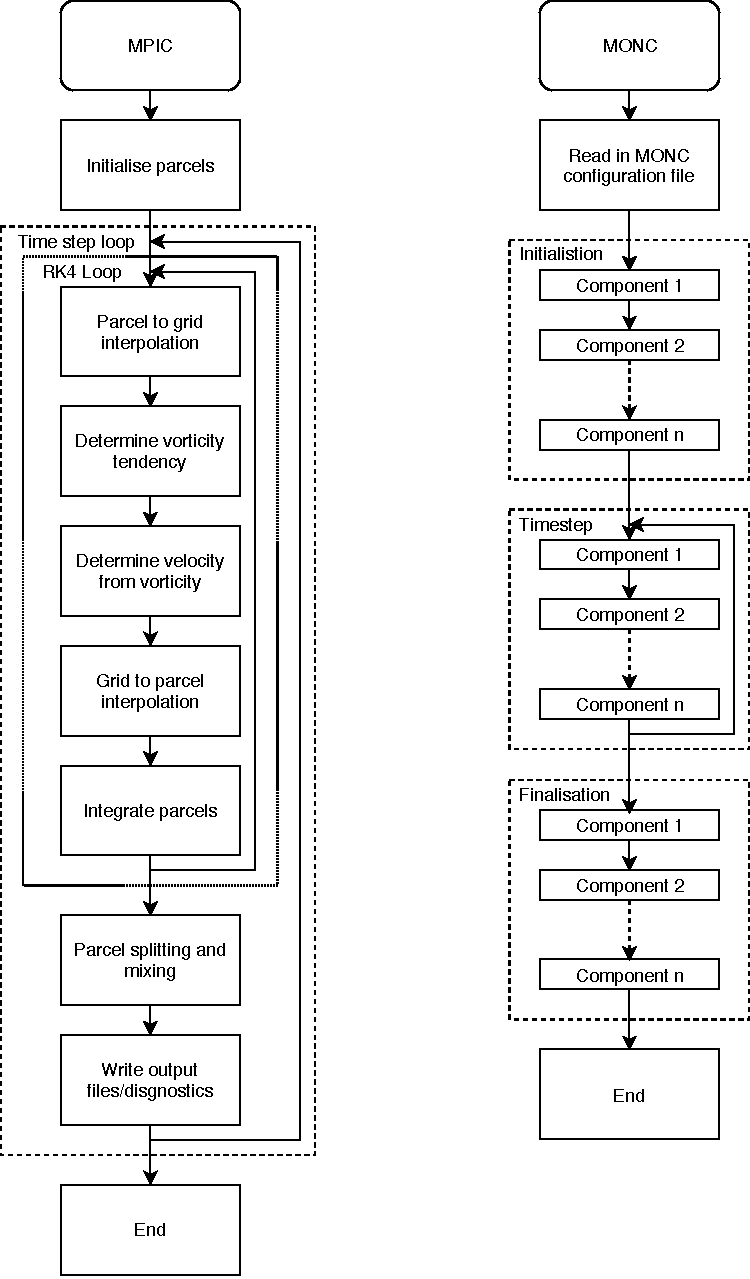
\includegraphics[scale=0.9]{pmpic_images/flowchart.pdf}
  \end{center}
  \caption{Flowcharts showing the structure of MPIC (left) and MONC (right).}
  \label{flowchart}
\end{figure}

\subsection{Proposed Technical Work}
The proposed work was to incorporate the parcel-based MPIC into MONC, producing a so called `Parallel Moist Parcel in Cell' (PMPIC) code, which scales beyond one node, permitting larger simulations to be carried out than are possible with MPIC. Incorporating MPIC into MONC is beneficial as MONC's layout makes it easy to implement new functionality into, and much of its functionalty can be used with minimal modifications to permit the MPI parallelisation of MPIC.
This also broadens the scope of MONC as it adds Lagrangian functionality, complimenting its existing Eulerian functionality.

The proposed work was split into four Work Packages:
\begin{itemize}
  \item WP1: MONC Model Extensions\\
  Modify the Model Core so that it is parcel-aware by implementing parcel-specific functionality. Additionally modify the Model State to contain parcel data. This work includes interpolation routines to interpolate to/from grids from/to parcels, haloswapping parcels between processes, Fourier transforms, operations on spectral variables and functionality to use the RK4 integrator.
  \item WP2: Dynamical Core implementation\\
  Implement various MONC components to provide the existing MPIC functionality. These components include a RK4 integrator, parcel splitting and merging, velocity inversion, and velocoty tendency.
  \item WP3: Diagnostics\\
  Implement parcel awareness into the I/O Server and some basic parcel data analysis operations.
  \item WP4: Testing, Validation and Training\\
  Testing and validation of the work carried out in WP1 to WP3. This Work Package will be carried out in parallel with WPs 1-3 where necessary. Additionally, provide an ARCHER Webinar to publicise the work carried out in the eCSE and advise potential users in PMPIC's use.
\end{itemize}
Throughout the project we aimed to include OpenMP functionality into PMPIC, making it a hybrid OpenMP/MPI code.
In the following sections we will refer to left/right as the -ve/+ve $x$ direction, down/up as the -ve/+ve $y$ direction, and bottom/top as the -ve/+ve $z$ direction.

\section{Technical Work Carried Out} \label{development}
We will now describe the technical work carried out in this project. It broadly falls under four categories: adding parcel properties into the Model State, implementing parcel functionality into the Model Core, writing components, and diagnostic routines. In the following subsections we will describe the work carried out in the four aforementioned categories, and will describe testing and validation applied to the code.

\subsection{Model State}
\subsubsection{Arrays vs Derived Datatypes}
\begin{figure}
  \begin{center}
    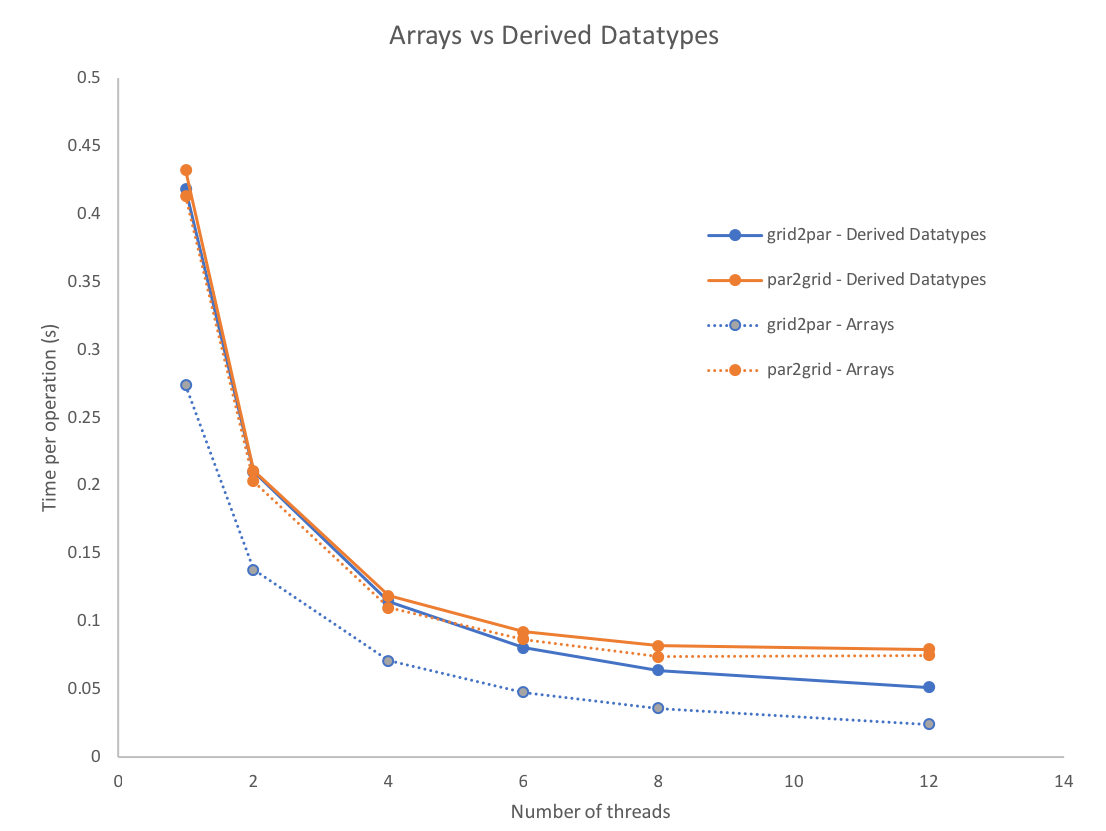
\includegraphics[scale=0.5]{grid2par.png}
    \caption{Comparison of the mean time per par2grid and grid2par operation for both \emph{array} and \emph{derived datatype} parcel descriptions.\label{grid2par_comp}}
  \end{center}
\end{figure}
Firstly, it is important to determine how to best represent parcels in PMPIC. There are two main ways this could be done: an array of a `parcel' derived data type containing all the parcel properties (hereby the \emph{derived datatype} approach), or several arrays, one for each parcel property (hereby the \emph{array} approach). The \emph{derived datatype} approach simplifies haloswaping, as one can simply send arrays of the $n$ parcel datatypes. If in future extra parcel properties are added, other than re-defining the parcel datatype, little to no work has to be done to change the existing parcel haloswapping routines. On the other hand, the \emph{array} approach allows a single parcel property for all the parcels (e.g. buoyancy) to be contigious in memory, which may result in performance gains when acting on a single parcel property, although parcel haloswapping is not so easy to implement.

Performance analysis of MPIC showed that a significant amount of the runtime is spent in the parcel interpolation routines. We therefore wish to choose a parcel representation that gives the best performance in these routines. In order to determine the optimal parcel representation we wrote basic parcel to grid (par2grid) and grid to parcel (grid2par) routines that could handle the \emph{array} approach and the \emph{derived datatype} parcel descriptions, and determined the mean time per operation for each interpolarion. A graph of the times per operation for a gridsize of $128^3$ using $2^3$ parcels per cell is displayed in Figure \ref{grid2par_comp}. It shows that grid2par takes roughly the same time using either method, but that par2grid is significantly faster using the \emph{array} decription. On average the \emph{array} description is $6\%$ faster for the par2grid operation, and $70\%$ faster for the grid2par operation. We therefore chose the \emph{array} parcel representation method due to its better performance.



\subsubsection{MPIC Data Representation}
In order to minimise the alterations to existing MONC code, we chose to place all the parcel related data into a \verb|parcels| derived datatype inside the model core so that they were separated from the rest of the data, and also clearly labelled as belonging to parcels. The various grids used by MPIC were chosen to be the existing \verb|prognostic_field_type| datatype and were simply added as additional members of this type into the model state.

In order to facilitate the possibility of adding additional parcel properties in the future, we implemented a two dimensional array of parcel properties in the \verb|parcels| datatype, indexed by parcel number, and the index of the property. This array is implemented into the parcel haloswapping routines (Section \ref{parcel_haloswapping}) so that newly added parcel properties are automatically haloswapped, and no additional work is needed to implement haloswapping for these new properties.

\subsection{Model Core}
With a description of the parcel data in the Model State, we could then move onto developing functionality into the Model Core.

\subsubsection{Parcel Interpolation}
The parcel interpolation routines form the backbone of MPIC, as they allow parcel properties to be interpolated onto the grid and vica versa. For par2grid/grid2par, a parcel's properties are trilinearly interpolated to/from the eight gridpoints surrounding that parcel. For par2grid, a grid point's value is derived from the weighted sum of \emph{all} the parcels in the eight cells surrounding it, whilst in grid2par a parcel's value is determined from the weighted sum of the values of the eight grid points surrounding it.

In MONC, where the domain in spatially decomposed, parcels on the edge of a domain will require to pass/retrieve values to/from a gridpoint belonging to a neighbouring process. For grid2par we perform a normal haloswap (adjacent processes' edge cells to the halo) and we can then interpolate onto parcels. This is not so simple in par2grid however, as we are moving parcel properties onto grid points via a sum. A \emph{reverse haloswap} is required, where we send a process' halo cells to adjacent processes, who then add it to the values in their own cells. This differs from regular haloswapping, which send regular cells to halo cells.

Due to the parallel decompositon of MONC (in the $x$ and $y$ directions), parcels are only influencers/influenced by halo cells in the right and upward edges of the process' domain. We hence only need to haloswap the right and upper edges of the grids as halo values in the downward and left edges are not needed. With this, and the fact that par2grid requires a special kind of haloswapping, we implemented our own grid haloswapping rather than try to modify MONC's existing haloswapping functionality. We produced two haloswapping routines, \verb|grid2par_haloswap| and \verb|par2grid_haloswap| for use in grid2par and par2grid respectively.

In order to validate our par2grid and grid2par routines, we constructed test cases consisting of linear profiles in $x$, $y$ and $z$ (or a combination of two or more directions) and ensured that we could recover the correct parcel/grid values from the interpolations. We chose linear profiles as the trilinear method is only guaranteed to produce the correct result for linear profiles.

\subsubsection{Parcel Haloswapping}\label{parcel_haloswapping}
As parcels are evolved in time they will move about the computational domain, and we therefore need to be able to pass these between individual processes' domains. In order to do this we carry out the following operations:
\begin{enumerate}
  \item Loop over all parcels in the process and flag the parcels that need to be transferred to neighbouring processes.
  \item For each neighbouring process, construct buffer arrays where the parcels that need to be sent to that process are stored.
  \item Send these buffers to each neighbour via a non-blocking send.
  \item Receive buffers from each neighbouring process, and unpack the parcels into the parcel arrays, backfilling into gaps left by sent parcels where applicable.
  \item Backfill parcels into any remaining holes left by sent parcels.
\end{enumerate}

In order to test parcel haloswapping, we implemented a basic Eulerian integrator component and a component to prescribe the parcel velocities, $\v{u} = f(x,y,z)$. We tagged parcels according to their starting position and integrated parcel trajectories for a number of timesteps and ensured that the end solution was identical regardless of the number of processes used. Velocity profiles tested included a constant velocity in various directions and a rotational velocity profile. An example of a test is shown in Figure \ref{parcel_haloswap}, where a series of parcels split between four processes is advected according to a rotational velocity field. The parcels are colour-coded by their initial process, and are successfully transferred between processes as they move around the computational domain.

\begin{figure}
  \begin{center}
    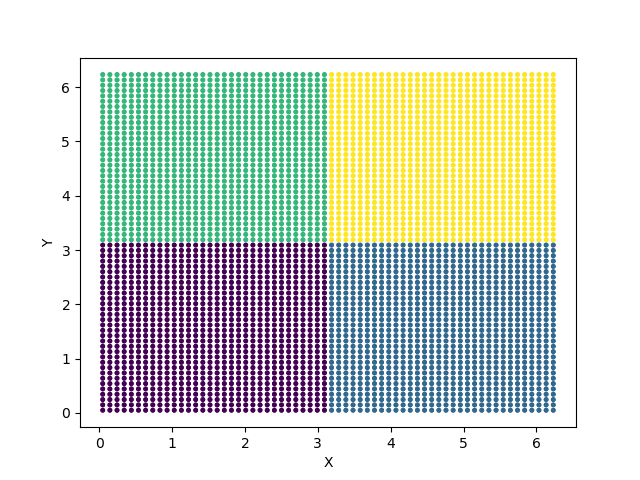
\includegraphics[scale=0.45]{pmpic_images/vel0.png}
    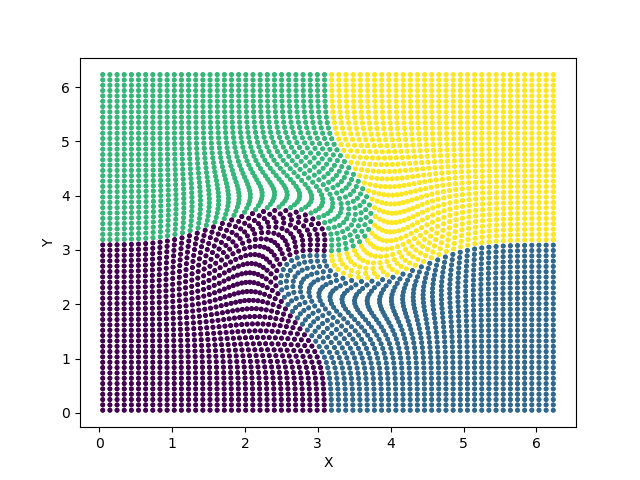
\includegraphics[scale=0.45]{pmpic_images/vel1.png}
  \end{center}
  \caption{Parcels coloured according to their initial process before (left) and after (right) being advected by a rotational velocity profile, demonstrating that the parcels have been successfully haloswapped between processes. \label{parcel_haloswap}}
\end{figure}

\subsubsection{Implementing functionality for a RK4 integrator}
MONC uses an Eulerian integrator, so per timestep each component is called once, and the model state is evolved at the end. In MPIC, which uses a RK4 integrator, several components would need to be called four times in seequence, correspending to each of the four steps in the RK4 integration. We thus had to modify the Model Core so that it knew to call a group of components a fixed number of times per timestep.

\subsubsection{Fast Fourier Transforms and Spectral Derivatives}
A number of MPIC's solvers use Fast Fourier Transforms (hereby FFTs) when calculating quantities. An existing MONC component also uses FFTs for a calculation, so we used the pre-existing FFT functionality from this component, but built it into the model core. MONC's FFT routines perform FFTs in the $x$ and $y$ directions using the FFTW library, leaving the $z$ direction in positional space. The grids are therefore transformed into semi-spectral space. MONC stores the complex output in double precision (real) arrays, where odd-numbered indices are the real part, and even-numbered indices are the imaginary part. As a real to complex FFT of $N$ points produces $N/2+1$ complex numbers, the resultant (global) transformed grids contain $N_x+2$, $N_y+2$ and $N_z$ cells in the $x$, $y$ and $z$ directions respectively. This means that for certain grid decompositions, a complex number (pair of reals in the array representation) can be split between two processes.

MPIC's solvers use spectral derivatives, that is, differentiation is carred out on a spectral variable. Mathematically, to do this we compute:
\begin{equation}
  F'(k) = 2\pi i k F(k),
\end{equation}
where $F(k)$ is the fourier transformed quantity, $F'(k)$ is the derivative of the quantity and $k$ is the wavenumber. To compute the second derivative we simply have
\begin{equation}
  F''(k) = -4\pi^2 k^2 F(k).
\end{equation}
In order to implement the first derivative we simply need to multiply each entry in the array by $2 \pi k$ and swap the real and imaginaty parts in each pair around to represent multiplying by $i$. As these pairs can be split between processes we need to send messages to swap these values. As the second derivative requires no swapping, this is simple to implement as all we do is multiply each entry in the array by $4 \pi^2 k$.

In order to verify the FFT routines we got them to compute FFTs functions with known fourier transforms, and compare the values. Similarly, we tested the spectral derivatives by taking the FFT of a known function, differentiating it, then taking the inverse FFT and ensuring it matched the analytical derivatives.

\emph{We note here that MPIC differs from MONC in that it takes FFTs in the $x$, $y$ and $z$. We however adopt the MONC approach in PMPIC and use a tridiagonal solver in the $z$ direction rather than a FFT solver. Please see Section \ref{inversion} for more details on the solver.}

\subsubsection{Timing routines}
In order to better quantify the performance of PMPIC, it was decided to implement timing functionality into the code. In order to do this we added a timing subroutine into the model core which components could register with, and report when they were entered and exited. This timing component could then report timing statistics at the end of the run so the user (and developer!) can get an indication of which parts of the code are the most time consuming.

\subsection{Components}
With the Model Core fuly parcel-aware, and general functionality required MPIC in place, components could then be implemented.

\subsubsection{Parcel/Grid Setup}
We first wrote some basic components that read in a config file and allocated memory for the parcels and grids. These used much of the existing MONC Model Core functionality for determining the parallel decomposition and grid properties. It was also important to produce a component that set up the parcels according to the initial condition. It was decided that this component would be user-supplied, and would set up the parcels as needed for the simulation. For the eCSE project we wrote a component that produces the initial condition for the spherical thermal described in \citet{Dritschel2018}.

\subsubsection{Basic I/O Routines}
Before work on WP3 where more sophisticated I/O would be developed, we wrote two basic I/O components. The first component was a parcel and grid writing routine, which would produce binary files for the grid and parcels, one file per process. The user could choose how often these files were created, and select whether they wanted to write files every $n$ timesteps, or every fixed time interval $dt$. The user could choose different writing frequencies for parcels and grids.
The second component was a component that read parcel files into memory, allowing a restart functionality for PMPIC. We designed this so that parcel files written by $m$ processes could be read in by $n$ processes so that a subsequent simulation could use a different number of processes from the previous one. Mindful to minimise stress on ARCHER's Lustre filessystem, the process with rank 0 opens each file sequentially and reads \emph{only} the creating process's location in the global domain from the file. It then broadcasts this to every other process which then open and read parcels in from \emph{only} the required files.


\subsubsection{RK4 Integrator}
 First we implemented a RK4 integrator. In order to do this we required storage for temparary arrays during the integration process. The quantities that are evolved are the vorticity and the parcel positions, whilst the gradients used are the velocities and vorticity tendencies. In total twelve temporary arrays are needed, six for the initial values of the parcel positions and vorticities, and six for the cumulative values for the positions and vorticity.

\subsubsection{Velocity Inversion}\label{inversion}
In order to solve for the velocity, we use the definition of vorticity,
$
  \gv{\omega} = \curl{\v{u}}.
$
Imposing that the flow is incompressible, $\div{\v{u}} = 0$, we can write $\v{u} = - \curl{\v{A}}$, where $\v{A} = (A,B,C)$, $\div{\v{A}} = 0$, is a vector potential. We can hence represent the vorticity as
\begin{equation}
  \gv{\omega} = \v{\nabla}^2 \v{A}.
\end{equation}
In semi-spectral space this equation becomes
\begin{equation} \label{vort2vel_eq}
  \pp{\v{A}}{z} - 4\pi^2 \v{K}^2 \hat{\v{A}}= \gv{\omega},
\end{equation}
Where $\hat{\v{A}}$ is the semi-spectral transform of $\v{A}$. This above equation when using finite difference derivatives in the $z$ direction, reduces to a tridiagonal problem that can be easily solved. We hence implemented a tridiagonal solver into PMPIC to be able to solve this equation.

Before we do this, however, we wish to correct the parcel vorticity, $\gv{\omega}_p$, to ensure that $\div{\gv{\omega}} = 0$. This formulation allows us to calculate the vorticity tendency in Section \ref{tendency}. To correct the vorticity we define a scalar $\chi$ where
$
  \gv{\omega} = \gv{\omega}_p - \grad{\chi}
$
Taking the divergence of this equation and setting it to zero we obtain
\begin{equation} \label{chi}
  \div{\gv{\omega}}_p = \nabla^2 \chi.
\end{equation}
This equation also reduces to a tridiagonal problem that can be solved with the tridiagonal solver.

The computational steps to invert the vorticity to produce the velocity field are:
\begin{enumerate}
  \item Apply the par2grid operation to the three components of the vorticity.
  \item Take FFTs of the three gridded components of the vorticity.
  \item Calculate $\div{\gv{\omega}}$ using spectral derivatives (in $x$ and $y$) and finite difference derivatives (in $z$).
  \item Obtain $\hat{\chi}$ by solving Equation \ref{chi} using the tridiagonal solver.
  \item Determine $\grad{\hat{\chi}}$ using spectral and finite difference derivatives (as required) and correct the vorticity.
  \item Use the tridiagonal solver to obtain $\hat{\v{A}}$ from Equation \ref{vort2vel_eq}.
  \item Calculate the semi-spectral velocity field from $\hat{\v{A}}$ and interse-FFT to obtain the velocity field.
  \item Inverse-FFT the corrected vorticity.
  \item Apply grid2par for the corrected vorticity and velocity.
\end{enumerate}

In order to test the velocity solver, we constructed an analytical form of $\gv{\omega}$ with a known $\v{A}$, and compared this to $\v{A}$ determined from the solver. Figure \ref{inversion_fig} displays graphs of the analytical solution of $\v{A}$ with the numerically determined $\v{A}$ for horizontal wavenumbers $(k_x,k_y)=(1,2)$.

\begin{figure}
  \begin{center}
    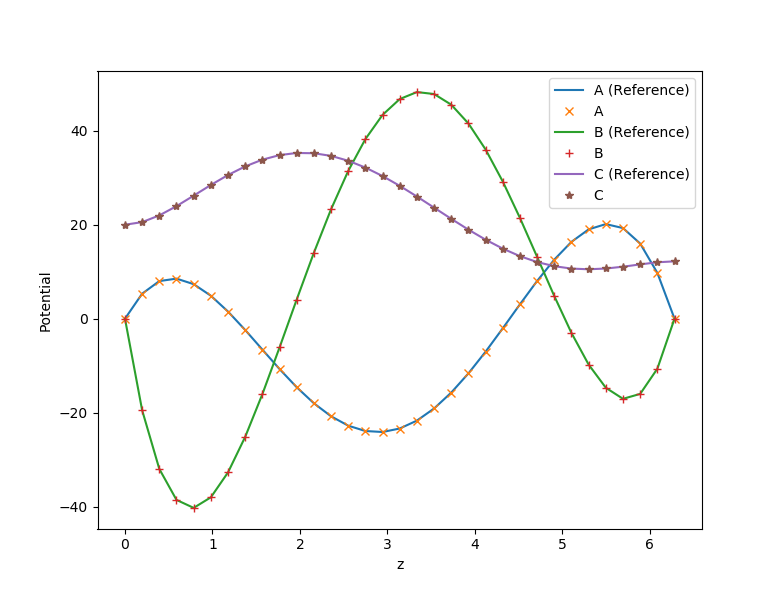
\includegraphics[scale=0.6]{pmpic_images/solution.png}
  \end{center}
  \caption{Comparison of reference (analytical) values of the velocity potential field against those determined from the solver.}
  \label{inversion_fig}
\end{figure}


\subsubsection{Vorticity Tendency}\label{tendency}
The vorticity tendency is defined by
\begin{equation}
  \pd{\gv{\omega}}{t} = ( \div{\v{F}},\div{\v{G}},\div{\v{H}}),
\end{equation}
where $\v{F} = \gv{\omega}u + b \uv{y} $, $\v{G}=\gv{\omega}v - b \uv{x}$ and $\v{H}=\gv{\omega}w$, where $b$ is the buoyancy, $(u,v,w) = \v{u}$, and $\uv{x}$, $\uv{y}$ are unit vectors in the $x$ and $y$ directions respectively.

The steps to calculate the vorticity tendency are as follows:
\begin{enumerate}
  \item Apply the par2grid operation on the buoyancy.
  \item Calculate the FFT of the buoyancy.
  \item For $\v{F}$, $\v{G}$ and $\v{H}$, determine their components in semi-spectral space.
  \item  Calculate the divergences of $\v{F}$, $\v{G}$ and $\v{H}$ using spectral derivatives to determine the vorticity tendency.
  \item Inverse-FFT the components of the vorticity tendency, then apply the grid2par to interpolate this onto the parcels.
\end{enumerate}

\subsubsection{Parcel Splitting and Mixing}
In order to simulate the cascade of energy to smaller scales which occurs during turbulence, MPIC splits parcels into smaller ones, then eventually merges them into surrounding parcels. We implemented this into PMPIC via two components, a splitting component and a mixing component.

Every parcel carries a quantity called the stretch, defined by
\begin{equation}
  \gamma_i(t) = \int_{t_i}^{t} \left(\gv{\omega}_i \cdot \d{\gv{\omega}_i}{t} \right)^{\frac{1}{3}} dt,
\end{equation}
where $t_i$ is the time the parcel came into existence. Parcels are split into two parcels when the stretch exceeds a value of 4. Upon splitting, the two child parcels have half the volume of their parent, their stretch is reset to zero, but their other quantities remain identical to the parent's. The two child parcels are separated by a distance $d = (2V_i/\pi)^{1/3}$ (where $V_i$ is the volume of the parent parcel) along the direction of the parent's vorticity vector. The PMPIC implementation of this is identical to the MPIC implementation save for a parcel haloswap operation which is applied at the end of the process to ensure that any child parcels that end out outside of the process' domain are sent to the appropriate process. In order to test this component we created a set of parcels, and for some set their stretch to a value above 4, then ensured that the child parcels had correct positioning and values.

Once a parcel's volume has been reduced (through multiple splittings) below a threshold value (chosen to be $(1/6)^3$ of the volume of a grid cell), this parcel is removed and its properties are added to surrounding parcels to ensure conservation of mass. This merging process prevents a runaway increase in the number of parcels in the simulation, and limits the number of parcels per gridcell to $6^3$. In addition to removal of small parcels, if a grid cell has too few parcels inside it, a new parcel is created in the centre of the cell, and `absorbs' the properties of adjacent parcels (once again to conserve mass and other fluid properties). The mixing procedure is very similar to a par2grid followed by a grid2par operation, with some intermediate steps:
\begin{enumerate}
  \item Loop through each parcel and determine which parcels are smaller than the threshold volume for splitting and hence need to be removed.
  \item Carry out a par2grid operation on the parcels that are to be kept. Also perform a par2grid operation on the parcels to be removed, creating grids of the \emph{residual} variables.
  \item Perform a par2grid and grid2par haloswap on the gridded values for parcels to be kept.
  \item If there are fewer than three parcels in a grid cell, create a new parcel in the centre of the cell and assign to it a volume of twice the minimum volume for a parcel, assigning properties to it proportional to a weighted sum of the gridded properties (from kept parcels) of the eight corner points of that cell. Adjust the residual grids to compensate for the transferred grid properties to the new parcel.
  \item Backfill parcels into positions of parcels that were removed.
  \item Now perform a par2grid and grid2par haloswap on the residual grid properties
  \item Finally perform a modified grid2par operation where the quantities from the residual grids are added to the existing parcel properties.
\end{enumerate}
It is important that both a par2grid and grid2par haloswap is performed on the grids of kept parcels \emph{before} the creation of new parcels in Stage 4. This ensures that grid cells on the edge of the computational domain have the correct grid values for interpolating onto the new parcels. Similarly, once the new parcels have been added, par2grid and grid2par haloswaps of the residual grids are required to ensure that these grids are correct for interpolation back onto the existing parcels.

In order to test parcel removal a number of parcels at random had their volumes reduced below the minimum volume threshold. Global volume-integrated quantities were determined for the grid and stored. After the mixing process was complete, the global volume-integrated quantities were re-computed, and compared against the original values to ensure that they were the comparable. In order to test adding in new parcels, a number of parcels were removed from a number of cells at random to reduce the parcel count below three in these cells. Then the global volume-integrated quantites were determined, the parcel creation process was carried out, then the new volume-integrated properties were compared to the old ones. For both methods it was found that the global quantities were conserved to a factor of $10^{-13}$ when half of the parcels were shrunk/removed.


\subsection{Diagnostics}
The original intention was to use the MONC I/O server to reduce parcel data from the simulations and write parcel/grid information to file. Unfortunately it became evident that parcels consume a large amount of memory and so allocating memory for parcels in an I/O server on a node would potentially require half of all the memory of that node, meaning we would need to run a simulation with a given number of compute processes on twice as many nodes if we were to use an I/O server. Without any I/O server, for simulations with grid resolutions of $256$, $512$ and $864$, we found a minimum of $3$, $43$ and $216$ nodes respectively were required to successfully run simulations. These node counts (especially for the larger gridsizes) are non-trivial, so using an I/O server would double this minimum number, and potentially double kAU usage. We therefore decided against using MONC's I/O server as its use could significantly increase the cost of running PMPIC simulations.

We instead focused on writing a parallel NetCDF writer component for the grids (so one file per timestep collectively written by every process). \textbf{STEEF's Bit}.

Due to the size of parcel checkpoint files (up to 2GB per process) we decided against creating an equivalent parallel NetCDF writing component, as the resultant files could be very large and therefore difficult to transfer. We instead focused on writing a visualisation script that could visualise a quantity (e.g. buoyancy) in a plane from the parcel properties. This is beneficial over simply obtaining this from the gridded variables as a higher resolution can be obtained using parcels. To do this, our script determines which files correspond to the regions in the global domain that are needed to construct the plane. Each required file is then read in and the relevant parcel properties are interpolated onto the plane to produce the image. For information on the specific interpolation method employed, please see \citet{Boeing2018}. An example of an image produced by the parcel visualiation script (and the corresponding image constructed from the grid variables) from a simulation with $32^3$ gridpoints is shown in Figure \ref{lowres}.

\begin{figure}
  \begin{center}
    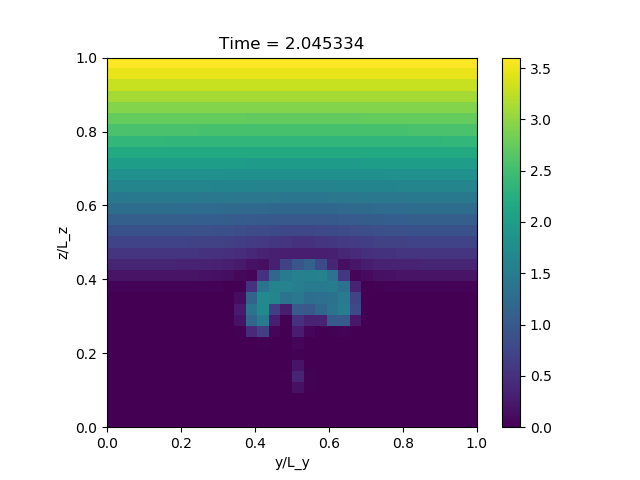
\includegraphics[scale=0.5]{pmpic_images/32grid.png}
    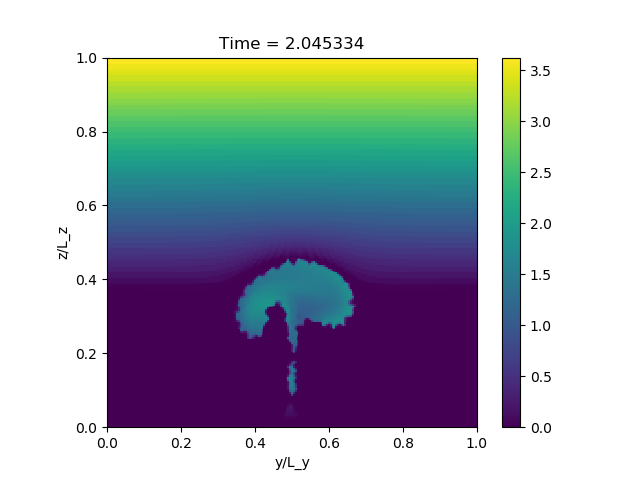
\includegraphics[scale=0.5]{pmpic_images/32parcels.png}
  \end{center}
  \caption{Comparison of the bouyancy in the $z-y$ plane for a $32^3$ grid cell simulation constructed from the gridded values (left) and from the parcels (right). It can be seen that images constructed from the parcels have considerably more detail as they are able to resolve sub-gridcell structure. \label{lowres}}
\end{figure}

\section{Performance Comparisons with MPIC and Scaling Tests} \label{performance}
In this section we will compare PMPIC performance with MPIC, and then go onto investigating how PMPIC performs at scale.

\subsection{Single Node Performance}

\begin{figure}
  \begin{center}
    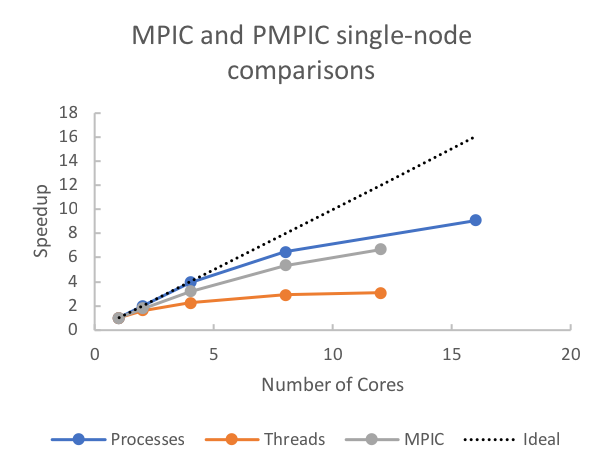
\includegraphics{pmpic_images/singleNode.png}
  \end{center}
  \caption{Speedup comparisons between MPIC and PMPIC using MPI processes and OpenMP threads.}
  \label{MPI-OMP-comp}
\end{figure}
In order to compare PMPIC with MPIC, we consider the performance of PMPIC on a single node, as MPIC (being parallelised solely with OpenMP) can only scale to one node. We ran a $128^3$ simulation for 8 time units, using 1, 2, 4, 8 and 16 MPI processes, and 1, 2, 4, 8 and 12 OpenMP threads. Figure \ref{MPI-OMP-comp} displays speedup graphs for MPIC, and PMPIC using MPI processes and OpenMP threads. PMPIC (using only MPI processes) produces the best speedup, with near ideal speedup to 4 MPI processes, then sub-ideal speedup to 16 processes. At 16 processes a speedup of 9.09 is achieved (parallel efficeincy of 57\%). MPIC achieves the second best speedup, with a speedup of 6.68 with 12 cores (parallel efficiency of 56\%). PMPIC's OpenMP performance is the worst, with a peak speedup of 3.05 at 12 cores (parallel efficiency of 25\%).

\begin{figure}
  \begin{center}
    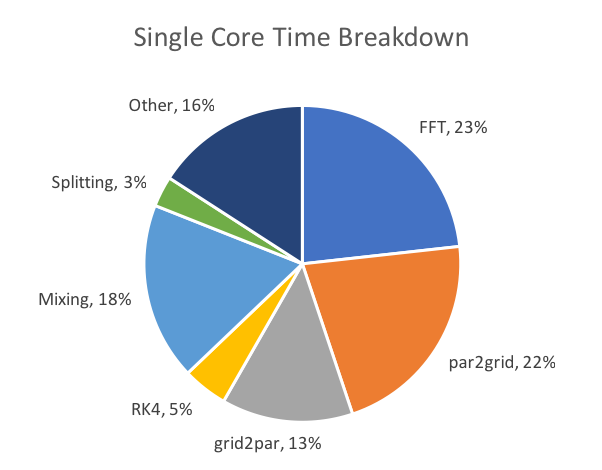
\includegraphics{pmpic_images/pie.png}
  \end{center}
  \caption{Fraction of the total runtime of each operation in PMPIC for a simulation using 1 core with $128^3$ gridcells.}
  \label{pie chart}
\end{figure}

\begin{figure}
  \begin{center}
    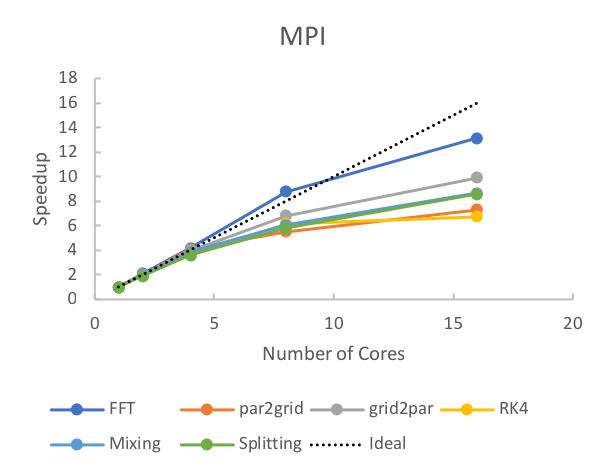
\includegraphics[scale=0.8]{pmpic_images/MPISingle.png}
    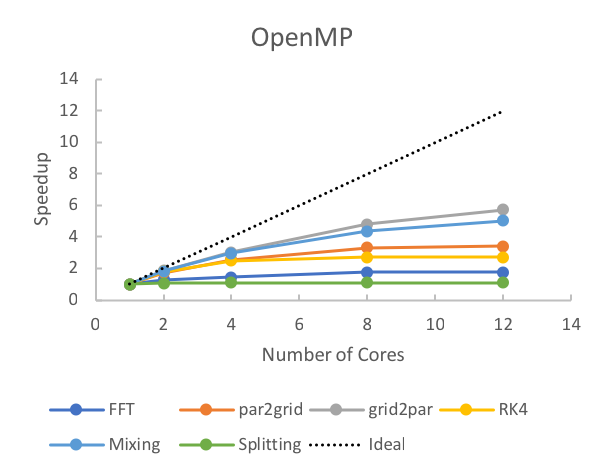
\includegraphics[scale=0.8]{pmpic_images/openmpSingle.png}
  \end{center}
  \caption{The speedup of the operations for MPI (left) and OpenMP (right)}
  \label{1 node operations}
\end{figure}

In order to determine the causes of the bad OpenMP scaling and poor MPI scaling beyond 4 processes in PMPIC, we consider the timings for each of the main operations carried out in PMPIC. First of all, let us consider the single-core case, and look at the relative times for each operation. Figure \ref{pie chart} displays the proportion of the runtime taken up by each operation. The single largest operation (by time) is the FFT operation, followed by par2grid and mixing. Parcel splitting is the least significant operation at only 3\% of the total runtime. Figure \ref{1 node operations} displays the speedups for OpenMP and MPI for each operation. For OpenMP, we find that parcel splitting and the FFT routines have the worst speedups. The mixing routines cannot be paralellised with OpenMP so the lack of a speedup is to be expected here. Also they take up a small proportion of the total runtime of a simulation so their poor scaling is of little concern. With the FFT routines - which consume the largese proportion of the runtime - although the execution of the FFTs and some data transposition is parallelised, the required \verb|MPI_Alltoall| communication step is not parallelisable, and so acts as a bottleneck in OpenMP. The next two poor performing operations are par2grid and the RK4 integrator. It is unclear why OpenMP performance is so poor here as these are completely parallelised via OpenMP. We suspect we need to tune the chunk size in the OpenMP \verb|DO| loops. Considering the MPI performance, we see that all operations scale well to 4 processes, and then scale less well beyond this, with the notable excepton of the FFT routines. This performance drop above 4 processes can be attributed to a load imbalance being introduced due to the domain decomposition, whereby some processes contain fewer parcels, so any operation involving parcels will have a load imbalance introduced. This is why the FFT operations, which are purely grid-based scales better than the other operations, which involve parcels. Figure \ref{parcel imbalance} displays the number of parcels per process as a function of timestep for 4 and 8 processes.

\begin{figure}
  \begin{center}
    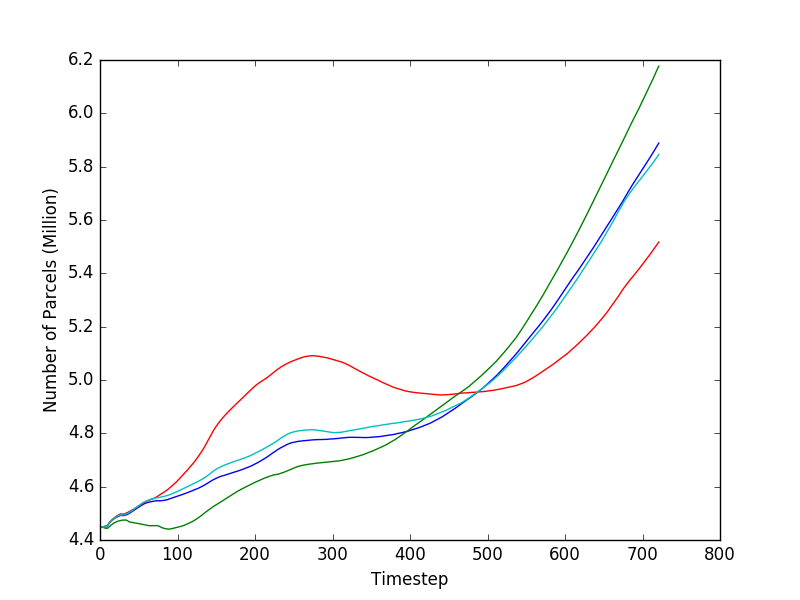
\includegraphics[scale=0.35]{pmpic_images/4p.png}
    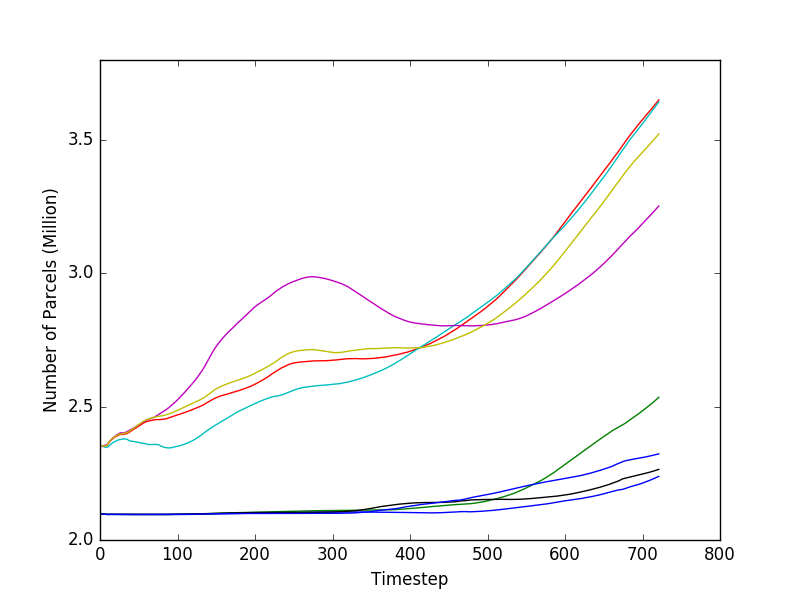
\includegraphics[scale=0.35]{pmpic_images/8p.png}
  \end{center}
  \caption{Number of parcels per process as a function of timestep for simulations with 4 (left) and 8 (right) processes, demonstrating that an imbalance of a factor of 1.6 between the number of parcels per process for the simulation with 8 processes.}
  \label{parcel imbalance}
\end{figure}

In terms of overall performance, MPIC was found to achieve 353,000 parcels operations per core per second, and 198,000 on 12 OpenMP threads. For a single core, PMPIC achieves 563,000 parcel operations per core per second and on 12 OpenMP threads it achieves 131,000 parcel operations per core per second (slightly less than MPIC), however on 16 MPI processes achieves 412,000 parcel operations per core per second, which is better performance than MPIC. Overall, despite achieving poorer OpenMP performance, using MPI PMPIC has better scaling and performance than MPIC.

\subsection{Performance at Scale}

\begin{figure}
  \begin{center}
    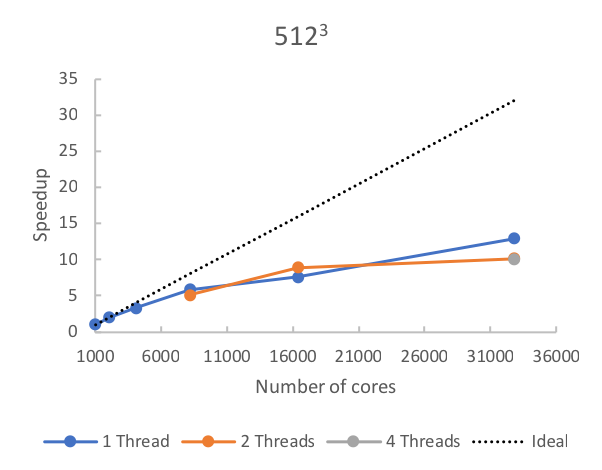
\includegraphics{pmpic_images/512.png}
  \end{center}
  \caption{Speedup of $512^3$ gridcell simulations with 1, 2 and 4 OpenMP threads.}
  \label{512 scaling}
\end{figure}
We now shall consider the performance of PMPIC for large simulations. We consider simulations with $512^3$ and $864^3$ gridcells respectively. Figure \ref{512 scaling} displays the speedup graph for the simulation with $512^3$ gridcells for 1, 2 and 4 OpenMP threads per process. With 1 thread per process, we find good scaling from 1024 to 8192 cores, and the scaling deteriorates from this point. Considering the speedup of the operations (Figure \ref{512 op}) we find that all the operations scale ideally up to 32768 processes except for the FFT operations, which do not scale beyond 2048 processes. It is clear therefore that the FFT routines (in particular the \verb|MPI_Alltoall| call) are a bottleneck for the simulations at this scale. In order to determine if OpenMP can help alleviate this (by reducing the number of MPI processes for a given number of nodes) we investigated some simulations with multiple OpenMP threads per process for larger core counts, which gave similar performance to the pure MPI simulations.

\begin{figure}
  \begin{center}
    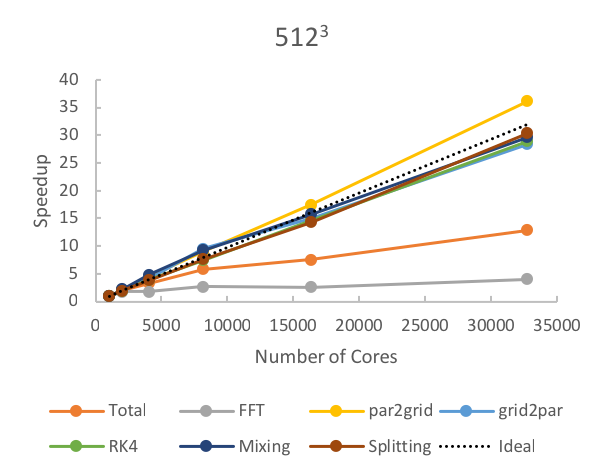
\includegraphics{pmpic_images/512ops.png}
  \end{center}
  \caption{Speedup of operations in $512^3$ gridcell simulations demonstrating that all the operations save for FFTs scale ideally.}
  \label{512 op}
\end{figure}

Figure \ref{864 speedup} displays the speedup for simulations with $864^3$ gridcells. It shows that we achieve good scaling to 20,736 MPI processes. Similar to the $512^3$ gridcell case, we find that all operations scale ideally for all core counts except for the FFT routines, which achieve a speedup of only 2.2 at 46,656 cores. We would have liked to have investigated the effects of OpenMP threads on the scaling of these simulations, however we had run out of budget on ARCHER so were unable to run further simulations. For $5184$ processes, we found that PMPIC achieved 140,000 parcel operations per core per second. We note that the load imbalance mentioned above - caused by processes having different numbers of parcels - is still present in these simulations, however as it is present in all simulations its effects are not visible in the speedup graphs. In these simulations the imbalance is typically a factor of 5. Given that the single core performance of PMPIC is 563,000 parcel operations per core per second, and the performance at scale is approximately 5 times lower, we believe that this load imbalance is the main contributng factor in the performance decrease. Figure \ref{864} displays the buoyancy in the $y-z$ plane for the a simulation with $864^3$ gridcells at $t=2, 4, 6$ and $8$.

\begin{figure}
  \begin{center}
    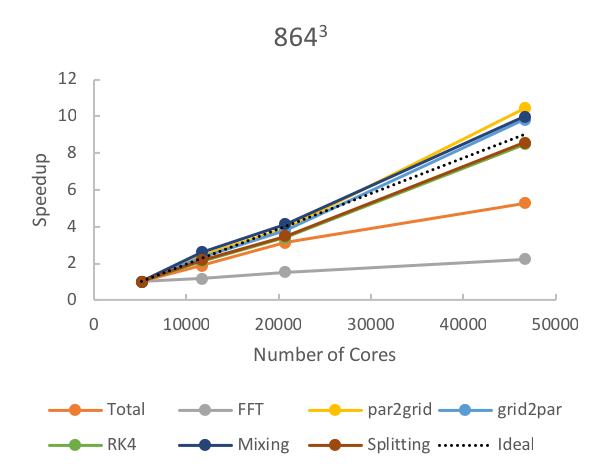
\includegraphics{pmpic_images/864.png}
  \end{center}
  \caption{Speedup of operations in $864^3$ gridcell simulations. Like shown in Figure \ref{512 op}, all operations scale ideally except for the FFTs.}
  \label{864 speedup}
\end{figure}




\begin{figure}
  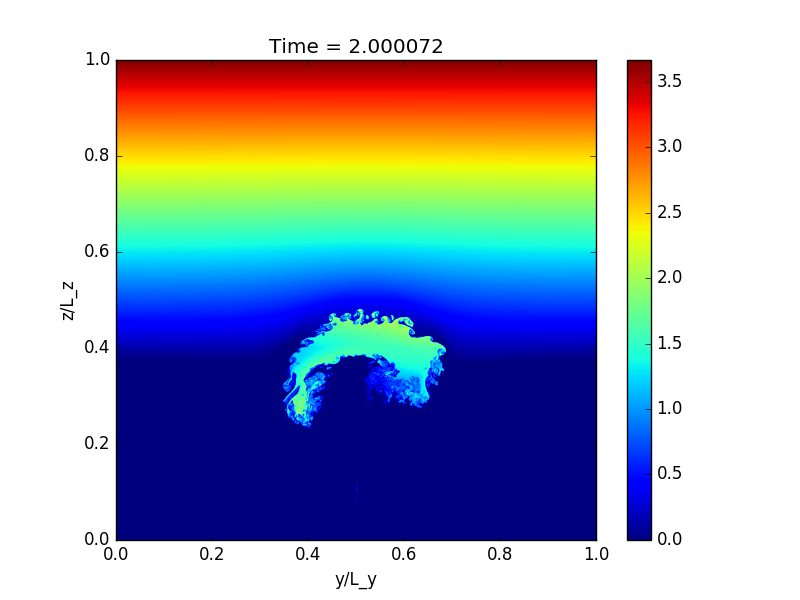
\includegraphics[scale=0.4]{pmpic_images/2.png}
  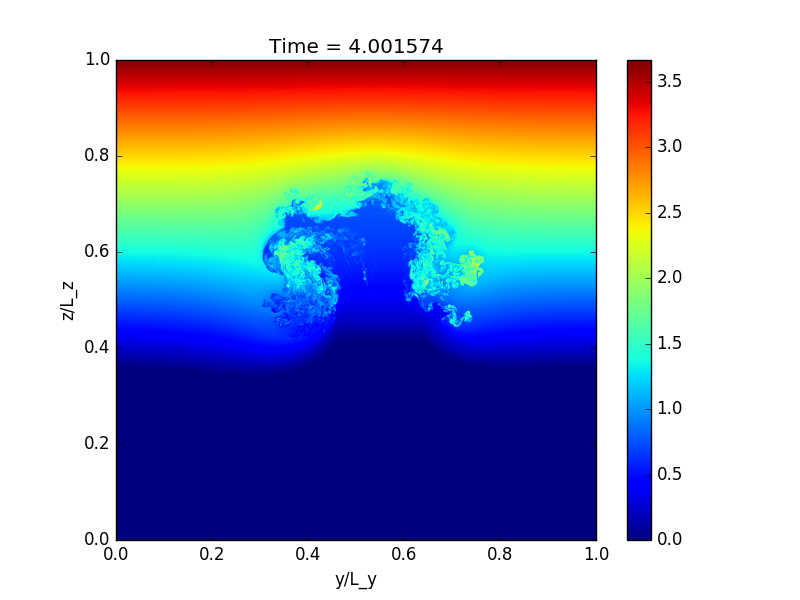
\includegraphics[scale=0.4]{pmpic_images/4.png}
  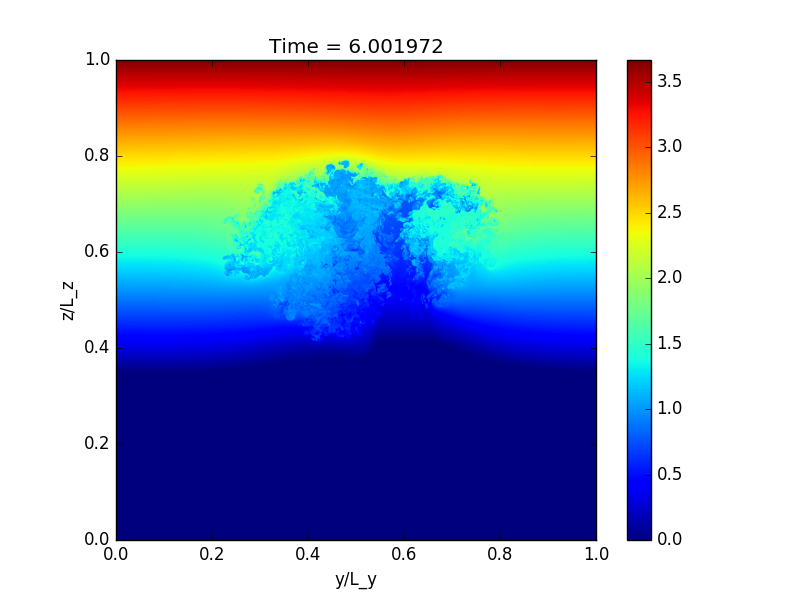
\includegraphics[scale=0.4]{pmpic_images/6.png}
  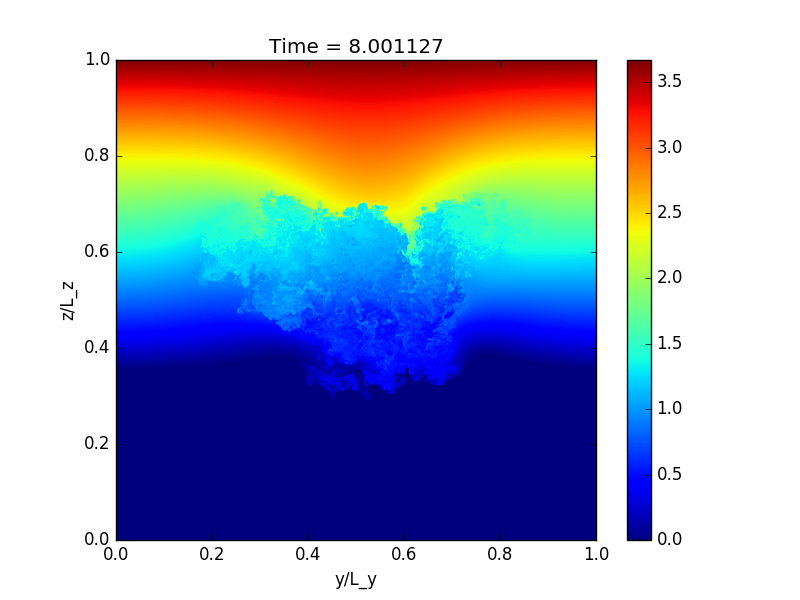
\includegraphics[scale=0.4]{pmpic_images/8.png}
  \caption{Example evolution of the buoyancy in a simulation with $864^3$ grid cells at t=2,4,6 and 8.}
  \label{864}
\end{figure}


\section{Discussion and Conclusions} \label{discussion}
In this project we implemented the `Moist Parcel In Cell' (MPIC) code into the `Met Office NERC Cloud Model' (MONC), allowing MPIC to benefit from MPI parallelisation, and making MONC parcel (particle) aware. We call this new code the `Parallel Moist Parcel In Cell' (PMPIC) code. The work involved modifying the MONC Model Core to include the basic parcel operations required for MPIC's functionality. This work included implementing grid-to-parcel and parcel-to-grid interpolation operations, as well as permitting MONC to use a 4th Order Runge Kutta integrator. We then wrote various MONC components to implement the physics of MPIC. Initially we had planned to modify MONC's I/O server to do in-situ analysis of the simulation data during a simulation, however due to memory limitations we decided against this as it could possibly double the computational cost of a simulation.

Comparing the single-node performance of PMPIC and MPIC, we found that the PMPIC (using MPI processes) scaled better than MPIC, however its OpenMP performance was poor, achieving a speedup of only 3 using 12 cores. MPI performance was limited by an imbalance in the number of parcels per process, due to the spatial decomposition of the simulation. Considering large simulations, we found that the PMPIC's performance was limited by the Fast Fourier Transform (FFT) routines, which did not scale well beyond a few thousand MPI processes. Other operations scaled ideally. Despite these limitations, we obtained good scaling (greater than 70\% parallel efficiency) of up to 8192 MPI processes (using a $512^3$ grid) and 20,736 processes (using a $864^3$ grid).

We note that although we did not implement the I/O server functionality, we did implement parallel NetCDF functionality for writing the grids to file. Although we did not have time to look into further work on in-situ analysis, we believe the way forward would be to write a MONC component (or series of components) that carries out analysis and I/O on the parcel data.

The load imbalance between processes affects the performance of PMPIC beyond 4 cores. This is due to the test simulation having a sphere of parcels in the centre with a higher number density ($4^3$ per cell compared to $2^3$ in the background), with most parcels being split in this central region. This results in some processes having many (up to 5$\times$) more parcels than other processes. Choice of a different initial condition with a more spatially uniform parcel distribution would help alleviate this issue, although our choice of initial condition here was constrained by the existing MPIC data which we wished to compare against. Future work could include implementing dynamic load balancing into PMPIC, although we note that this would be a major undertaking, as much of MONC's model core would need to be re-written to deal with dynamically changing each process' local grid size during runtime.

OpenMP performance was found to be poor in PMPIC. The worst performing operations were the FFTs (un-parallelisable), the Runge Kutta integrator and the grid2par interpolation. Future work would be to investigate if re-factoring these operations, or by changing chunk sizes can lead to better performance. With better OpenMP performance, we may be able to partially overcome MPIC's FFT scalability issues by using fewer MPI processes per node, hence decreasing the number of processes involved in the all-to-all communications.

For large simulations, are by far the most significant cause of poor scaling. Minimising the use of FFTs should therefore improve PMPIC's scaling. In PMPIC, FFTs are used in two different places. In the velocity inversion, the velocity is calculated using a FFT solver, whereby the solution is determined in semi-spectral space and then transformed back into positional space. Many spatial derivatives are also calculated in Fourier space, then transformed back into positional space. Implementing a solver that does not use Fourier transforms, and/or swapping Fourier derivatives with finite difference derivatives should therefore aid scalability to many tens of thousands of MPI processes.

In summary, the work in this eCSE project has allowed the Moist Parcel In Cell method to scale beyond one node, up to many thousands of cores, and allows more detailed simulations to be carried out, allowing better science to be carried out.


\section*{Acknowledgements}
This work was funded under the embedded CSE programme of the ARCHER UK National Supercomputing Service (http://www.archer.ac.uk)


\bibliographystyle{agsm}
\bibliography{refs}

\end{document}
